\documentclass[a4paper,12pt]{article}


% add more packages if necessary
\usepackage{xspace}
\usepackage{graphicx}
%\usepackage{xcolor}
\usepackage{hyperref}
\usepackage{amsmath}
\usepackage{enumitem}


% TODO: Add your group name
\newcommand{\groupname}{Ravioli\xspace}


\title{
Project Report \\
Group \groupname \\
\vspace{5mm}
\large Java and C\# in depth, Spring 2014
}
\author{
% TODO: Add your names here
Michael Bang (\texttt{mbang@student.ethz.ch}) \\
Pascal Fischli (\texttt{fischlip@student.ethz.ch}) \\
Vladimir Grozman (\texttt{grozmanv@student.ethz.ch})
}
\date{\today}



\begin{document}
\maketitle

\section{Introduction}

This document describes the design and implementation of the \emph{Personal Virtual File System} of group \emph{\groupname}. The project is part of the course \emph{Java and C\# in depth} at ETH Zurich. The following sections describe each project phase, listing the requirements that were implemented and the design decisions taken. The last section describes a use case of using the \emph{Personal Virtual File System}.

% PART I: VFS CORE
% --------------------------------------

\section{VFS Core}
VFS Core is the first step towards a Personal Virtual File System. It operates on virtual disks, of which each one is stored in a single file in the host file system. Its API not only offers functionalities to create, mount and delete virtual disks, but also to operate inside opened disks. This ranges from basic console operations, like navigating through directories, renaming and removing, to the virtual disk operations of importing and exporting directories, files or both together.\newline
The most important task in the process of creating the VFS Core is the design of the storage structure in the virtual disk files. The main aspect in this is efficiency. Not mainly in speed, but in usage of the available space. Two basic approaches are storing the files in one block, which of course could result in lots of space lost due to fragmentation, or splitting files into parts of predefined size that are always linking to the next part, resulting in a very space efficient but most likely slower system.


\subsection{Requirements}
In this part we indicate and describe what requirements we have implemented. We also list the main software elements involved in the respective implementation.

\begin{enumerate}
	\item The virtual disk is stored in a single file in the host file system. The creation happens in the creators of \texttt{JCDFAT}, which are creating a FileStream for the new file that is then written to in the creators of \texttt{JCDFAT}.
	\item The creation of virtual disk files happens in method \texttt{Create(string hfsPath, ulong size)} of class \texttt{JCDFAT}. The parameters specify the location and the initial size.
	\item Several virtual file systems on the host are allowed. Creation and opening, which is done with method \texttt{Open(string hfsPath)} of class \texttt{JCDFAT}, can happen an unlimited amount of times and with the file at any place on the host file system.
	\item Virtual disks can be disposed from the host file system, which can be done through the method \texttt{Delete(string hfsPath)} of class \texttt{JCDFAT}. Only files containing a virtual disk that can be opened are disposable through this.
	\item On a mounted VFS files and directories can be created, deleted and renamed with the methods \texttt{CreateFile(ulong size, string path, bool isFolder)}, \texttt{DeleteFile(string path, bool recursive)} and \texttt{RenameFile(string vfsPath, string newName)} in class \texttt{JCDFAT}.
	\item For basic navigation functionalities going to a specific location can be done with method \texttt{SetCurrentDirectory(string path)} in class \texttt{JCDFAT}. To support that, listing of files and directories can be done with the method \texttt{ListDirectory(string vfsPath)} in class \texttt{JCDFAT}, which is called by the method with the same signature in class \texttt{JCDFAT}.
	\item Moving of files and directories can be done with method \texttt{MoveFile(string vfsPath, string newVfsPath)} and copying with method \newline
	\texttt{CopyFile(string vfsPath, string newVfsPath)} in \texttt{JCDFAT}. Both preserve the internal file/directory hierarchy.
	\item Files and directories can be imported from the host into the virtual file system. This is done through method \texttt{ImportFile(string hfsPath, string vfsPath)} in \texttt{JCDFAT} which is then calling \texttt{ImportFolder(string hfsFolderPath, string vfsPath)} or \texttt{ImportFile(Stream file, string path, string fileName)} in \texttt{JCDFAT}.
	\item Exporting of files and directories from the virtual to the host file system is done in methods \texttt{ExportFile(Stream outputFile, JCDFile file)} and \texttt{ExportFolderRecursive(JCDFolder folder, string hfsPath)} in \texttt{JCDFAT}.
	\item How much space is free in the virtual disk can be queried and is calculated in method \texttt{GetFreeSpace()} in \texttt{JCDFAT}, which is multiplying the number of free blocks times the block size. The occupied space can be queried too and is calculated in method \texttt{OccupiedSpace()} in \texttt{JCDFAT} which is subtracting the free space from the virtual disk size.
\end{enumerate}

\subsubsection{Bonus points}
We've implemented two of the bonus features of this milestone. The first one is "Elastic disk". Our virtual disk initially takes up only the space required by the meta data (and FAT), and thereafter expands itself as needed when importing files. We currently have an untested implementation of automatic shrinking of the virtual disk.\\
The second bonus feature we've implemented is "Large data". This feature is implemented by using buffers of a predefined, constant size, when reading/writing files to/from the file system, instead of having the whole VFS in memory. The current implementation uses quite big buffers (100 MB), trying to mitigate the problem of constantly reading and writing from different parts of the hard disk.


\subsection{Design}
We decided to take a lot of inspiration from the FAT file system
\footnote{http://en.wikipedia.org/wiki/File\_Allocation\_Table}, also naming our file system JCDFAT. The overall structure of JCDFAT can be seen on Figure \ref{fig:block_structure}.\\
\\
The smallest unit of allocation in JCDFAT is one block, which currently is $2^{12}$ bytes (4KB).\\
\\
The first block of the file system contains meta data (see Figure \ref{fig:meta_data}). Even though the meta data currently only is 28 bytes, it has a full block allocated to it, as described above.\\
\\
The next block(s) contain(s) the File Allocation Table (FAT). Depending on how large the file system is, the FAT will span one or more blocks.
Since we're using 32 bit integers, and blocks of size 4KB, each FAT block allows us to address 4MB. This means that the smallest JCDFAT file system allowed is 4MB. It also means that the largest JCDFAT file system possible theoretically is 16 TB, but due to an implementation detail, it currently is 2 TB. The size of the FAT is \emph{included} in the size of the file system. The FAT takes up around 1/1024th of the file system; this means that if the file system is 16 TB, the FAT will be 16 GB.\\
There is no bound on the size of individual files, except the size of the file system.\\
\\
The two blocks following the FAT are reserved for the root directory and the search file. The root directory is the root folder of the file system. The search file is the file in which we wish to store meta data for indexing the file system, allowing us to implement file search in milestone 2 of the project.
\begin{figure}[ht]
    \begin{verbatim}
                File system structure
          (`|` represents a block boundary)

| Meta data | FAT block(s) | Root directory | Search file |
| data | data | data | data | data | data | data |  data  |
                        . . .
| data | data | data | data | data | data | data |  data  |
    \end{verbatim}
    \caption{Block structure of the JCDFAT file system.}
    \label{fig:block_structure}
\end{figure}

\begin{figure}[ht]
    \begin{verbatim}
Meta data
                         Size
+-----------------------+
| Magic number          | 4B
+-----------------------+
| Block size in         | 4B
| power-of-2 bytes      |
+-----------------------+
| Number of FAT blocks  | 4B
+-----------------------+
| Free blocks           | 4B
| (without expanding)   |
+-----------------------+
| First free block      | 4B
+-----------------------+
| Root directory block  | 4B
+-----------------------+
| Search file block     | 4B
+-----------------------+

Total size: 28 B
    \end{verbatim}
    \caption{Meta data for the JCDFAT file system.}
    \label{fig:meta_data}
\end{figure}
~\\
We use a structure called JCDDirEntry (see Figure \ref{fig:directory_entry}) to represent files on disk. Each directory entry is 256 bytes, meaning that we can have $\frac{2^{12}}{2^8} = 16$ entries in each block. Since the smallest unit of allocation is 4 KB, a folder takes up at least 4 KB of space. More generally, a folder takes up $\text{ceil}(\text{entries} / 16) * 2^{12}$ bytes.\\
\\
As can be seen on Figure \ref{fig:directory_entry}, the maximum length of a file name is 240 bytes. The string is interpreted as unicode, though, which means that the length of the file name is at most 120 characters.

\begin{figure}[ht]
    \begin{verbatim}
JCDDirEntry
                 Size
+---------------+
| Name          | 240B
+---------------+
| Size          | 8B
+---------------+
| isFolder      | 4B
+---------------+
| First block   | 4B
+---------------+

Total size: 256B
    \end{verbatim}
    \caption{Structure of a directory entry stored on disk in JCDFAT.}
    \label{fig:directory_entry}
\end{figure}

\subsection{File system events}\label{file-system-events}
The following is an explanation of how the implementation of our file system behaves in different scenarios.\\
\\
In the following we assume that there is always enough free space, and that the source and destination files and folders exist/don't exist as required.\\

\subsubsection{Finding a specific folder or file}\label{finding-a-specific-folder-or-file}
    \begin{itemize}
        \itemsep1pt\parskip0pt\parsep0pt
        \item{Starting at the root folder, recursively identify the directory entry}
          of the next folder specified by the given path.
        \item{Once the parent folder of the specified file or folder has been found,}
          find the specified file or folder.
    \end{itemize}

\subsubsection{Allocating space for a file}\label{allocating-space-for-a-file}
    \begin{itemize}
        \itemsep1pt\parskip0pt\parsep0pt
        \item{Figure out how many blocks the file requires,}
          $ceil(\frac{\text{size in bytes}}{2^{12}})$.
        \item{Starting from the first free block, walk the FAT in increments of 1, chaining free blocks.}
        \item{Mark the last used block as `end of chain'.}
    \end{itemize}

\subsubsection{Creating a file or folder}\label{creating-a-file-or-folder}
    \begin{itemize}
        \itemsep1pt\parskip0pt\parsep0pt
        \item{Allocate enough blocks to store the file. This is done by finding free entries in the FAT and chaining them.}
        \item{Store the file in the newly allocated blocks.}
        \item{Write a directory entry in the destination folder.}
    \end{itemize}

\subsubsection{Deleting a file (or folder)}\label{deleting-a-file-or-folder}
    \begin{itemize}
        \itemsep1pt\parskip0pt\parsep0pt
        \item{(Loop over all files/folders and perform delete file.)}
        \item{Starting from the first block of the file, walk the FAT chain and delete all entries.}
        \item{Delete the directory entry from the parent folder.}
    \end{itemize}

\subsubsection{Moving a file or folder}\label{moving-a-file-or-folder}
    \begin{itemize}
        \itemsep1pt\parskip0pt\parsep0pt
        \item{Move the file entry from the source folder to the destination folder. (File contents are not actually moved.)}
    \end{itemize}

\subsubsection{Renaming a file or folder}\label{renaming-a-file-or-folder}
    \begin{itemize}
        \itemsep1pt\parskip0pt\parsep0pt
        \item{Rewrite the name in the file's directory entry.}
    \end{itemize}


% PART II: VFS Browser
% --------------------------------------

\section{VFS Browser}
In this part of the project we're creating one or several user interfaces that are more sophisticated than the console client from the previous part, which means Graphical User Interfaces (GUI), for the VFS core. We decided to create a Windows desktop client and a web application written in ASP.NET. The browsers support both mouse and keyboard navigation. \newline
The clients offer all of the previously created operations of the VFS core and additionally a functionality to search for file/directory names with the options search location and case sensitivity.


\subsection{Requirements}
In this part we indicate and describe what requirements we have implemented. We also list the main software elements involved in the respective implementation. When requirements are described for both browser clients separately, we do so first for the desktop (a) and then the web client (b).

\begin{enumerate}
	\item The platforms we have created our browsers for are the Windows desktop and web (ASP.NET).
	\item
		\begin{enumerate} [label={(\alph*)}]
		\item All operations from VFS core are supported, some through buttons, especially operations on VFSs, but most through the list view, which is the main component of the browser, and its menu. The event handling is done mostly in MainForm.cs and the other Form classes.
		\item All operations from VFS core are supported, mostly through buttons. The event handling is done mostly in\newline
		Default.aspx.cs.
		\end{enumerate}
	\item
		\begin{enumerate} [label={(\alph*)}]
		\item In the list view single and multiple items can be selected. The operations where this multiple selection makes sense are then run on all those items.
		\item Same as for desktop.
		\end{enumerate}
	\item
		\begin{enumerate} [label={(\alph*)}]
		\item Keyboard navigation in the application is done mostly through the TAB key. In the list view going to child folders is done through pressing ENTER when a folder is selected. Going back can be done trough the Back-Button or the BACKSPACE key. Common Windows key functionalities (e.g. Delete)as well as combinations (e.g. Ctrl+C, Ctrl+X, Ctrl+V, Ctrl+A) are all supported.
		\item All header links in the web ui have keyboard shortcuts that are accessed with Alt + the underlined character (in Chrome, the modifier may be different in other browsers). All buttons in the file browser similarly have a keyboard shortcut that is written in brackets. The UP button is accessed with Alt + U. All other buttons are accessed with the TAB key.
		\end{enumerate}
	\item
		\begin{enumerate} [label={(\alph*)}]
		\item Mouse navigation is supported in the expected way. In the list view double click on a folder means going into this folder. Going to the parent folder can be done by clicking on the Back-Button.
		\item Single click on a folder to enter it, click the up button to go to the parent folder.
		\end{enumerate}
	\item
		\begin{enumerate} [label={(\alph*)}]
		\item Search can be done by entering the file name into the text box at the top right corner and then pressing ENTER. Selection of the search options can be done in the menu that appears when a click on the v-Button besides the text box happens.
		\item The search box is above the file browser. There are checkboxes to restrict the search to the current folder and to do case sensitive search. To search in the whole VFS, go to the root folder.
		\end{enumerate}
\end{enumerate}

\subsubsection{Bonus points}
As a general bonus feature we have implemented browsers for two different platforms. The platform specific implemented bonus features are:
		\begin{enumerate} [label={(\alph*)}]
		\item In the desktop client we have implemented especially nice-to-have features like drag-and-drop. Inside of the list view, dragging with the left mouse button results in a move and with the right mouse button in a copy operation. Dragging from the Windows Explorer and dropping into the list view results in an Import. Dragging an item of the list view and dropping it outside of this view results in an Export.
		\item The existence of the web client.
		\end{enumerate}

\subsection{Design}

\subsubsection{Search functionality}
\label{sec:search_functionality}
In implementing search functionality on a file system, there are some decisions to be made. There are many different data structures to use, and different ways to use each data structure. In this project, we decided to optimize our implementation for full file-system search, i.e. looking for a file name throughout the whole file system. There, of course, are trade-offs being made when making decisions like the one just mentioned; optimizing for full-file system search has an impact on the time it takes to search through only a small subset of folders of the file system. In our implementation, it requires (in the order of) the same amount of operations to search through the entire file system as it does to search through only a single folder. This is a fact that we were aware of when making the decision, and found to be acceptable. It would be possible to have multiple data structures, each optimizing for a different type of search, but we decided to go with just one. Having multiple data structures adds much more complexity and overhead, both w.r.t. processing power and storage. To further optimize search performance, we also decided to keep an always-updated index of all files on the file system, trading a small downgrade in performance when importing and creating files for a vast upgrade in performance when searching for files.\\
We found that B+-trees are a perfect match to implement an efficient full-file system search. Thus, our implementation relies on this data structure. We did not implement B+-trees ourselves, but sought help from the open source community, where we found an implementation we could use called `bplusdotnet'. The code for this project can be found at \url{https://github.com/benaston/BTree}.\\
\\
The implementation of B-trees we use, `bplusdotnet', uses two files for storage; one for storing the data structure and one for storing the actual data we put in the nodes of the tree. We decided to store these two files in the virtual file system itself, in order to comply with the requirement that the virtual file system should span only one file on the host file system. This means that additional storage space is required for storing the B-tree data structure on the virtual file system, and makes it more difficult to predict exactly how much space is required when adding a new file. This has the implication that, even though there may be X bytes of free space on the drive, it might not be possible to import a file of X bytes because of the metadata that is also written to the file system.\\
\\
The implementation of the search functionality almost solely resides in the namespace `vfs.core.indexing', which wraps the implementation of B+-trees we use. This implementation is described further in Section \ref{sec:integration} because this mostly consisted of integration work.


\subsubsection{Desktop client}
The most notable design decision was to make a clean separation between the View part, where event handling from the MainForm is done, and the Control part that is accessing the VFS core functionalities. In order to do this, we have defined a class VFSSession.cs which is the only class in the client that is referencing vfs.core. It contains a JCDFAT object, which represents an open VFS, and mostly calls methods of this object to fulfill its tasks. On the other hand, no Forms functionality is used in it, which makes this class easily reusable for other clients.

\subsubsection{Web client}

The web client largely reuses the VFSSession class from the desktop client, though some changes were necessary because of differences in error handling and data binding. One important difference from the desktop client is that logging in and out is unified: after logging in, you can open, close or retrieve VFSes, all while staying logged in.

\subsection{Integration}
\label{sec:integration}
In order to integrate file search into JCDFAT, all we had to do was to add and maintain nodes in the B-tree when importing, renaming, moving, and deleting files on the virtual file system. These changes are not very interesting to comment on here, and make up only around a total of 30 lines of code in the classes JCDFAT, JCDFile, and JCDFolder. The only real integration work we had to do in this milestone, was to integrate the open source project `bplusdotnet' into our project.\\
\\
We had three obstacles to overcome during the integration of bplusdotnet into our project:
\begin{itemize}
    \item bplusdotnet doesn't provide support for having multiple keys with the same value.
    \item bplusdotnet writes its data to the host file system.
    \item bplusdotnet doesn't allow for case insensitive search.
\end{itemize}
In the following we describe how we overcame these three obstacles.\\
\\
In solving the first obstacle, we started out with implementing a wrapper (vfs.core.indexing.FileIndex) for the class SerializedTree of bplusdotnet. SerializedTree implements a B+-tree which maps unicode keys (which our file names are) to serializable objects. As already mentioned, SerializedTree doesn't support having multiple keys with the same value. But it does support using serializable objects as values, and since arrays of serializable objects are also serializable, our solution was to create a serializable class (vfs.core.indexing.IndexedFile) and use an array of this class as values. Our wrapper class (FileIndex) then implements the logic required to add and remove items from the array used as value in the B-tree.\\
\\
Since bplusdotnet uses instances of Stream for writing data to disk, we figured that the correct way to solve our second problem was to create a class which implements the Stream interface on our virtual file system. This class can be found in vfs.core.JCDFileStream. After having implemented JCDFileStream, we realized that it might also be useful for the 3rd milestone of the project, and so were even more happy with our solution.\\
\\
Even though the third obstacle wasn't the most difficult one to overcome, it probably was the most time consuming. Here, we decided to pull up our sleeves and give something back to the open source community; we went through the codebase of bplusdotnet and added support for case insensitive key comparisons. Since these modifications don't really have anything to do with our own project, this will not be described


% PART III: Synchronization Server
% --------------------------------------

\section{Synchronization Server}
In the last step of this project we are expanding the system from the previous steps so that users can easily distribute VFS files and work with a single disk on multiple machines. To do that a Synchronization Server has to be created and the existing clients have to be modified and extended accordingly.\newline
The server is supposed to keep track of users and their VFS files, as well as of changes to synchronized files. These changes are sent to clients that have the same file open instantly and are additionally stored for future retrieval.


\subsection{Requirements}
In this part we indicate and describe what requirements we have implemented. We also list the main software elements involved in the respective implementation.

\subsubsection{Browser}
\begin{enumerate}
	\item Both browsers allow the user to create new accounts or to log in to an existing account. The methods that are used for this are \texttt{LogIn(string username, string password)} and \texttt{Register(string username, string password)} in class \texttt{JCDVFSSynchronizer}.
	\item The browsers have an offline mode when a synchronized VFS file is opened but the user is not logged in. Logging in again will send the changes made while offline, as well as retrieve missing changes from the server. This happens in the \texttt{LogIn(string username, string password)} of class \texttt{JCDVFSSynchronizer}.
	\item Unsynced (open) VFS files can be added to logged in user accounts and also removed from them. This happens through the methods \texttt{AddVFS()} and \texttt{RemoveVFS()} of class \texttt{JCDVFSSynchronizer}.
	\end{enumerate}

\subsubsection{Server}
\begin{enumerate}
	\item The server maintains a table with the registered unique user names and their according password. The methods to do so are \texttt{Register(string name, string password)} and \texttt{Login(string name, string password)} of ther server's database class \texttt{JCDSynchronizerDatabase}.
	\item Changes coming from the clients to the server are executed locally in the respective method of \texttt{JCDSynchronizerDatabase} and then stored in the database in method \texttt{addChange(int eventType, long fileId, byte[] data)} of the same class. If there is another browser that has the changed VFS open, the change is sent to this client through methods \texttt{SendGroupMessage(HubCallerContext context,...)} of the hub class \texttt{JCDSynchronizerHub}.
	\end{enumerate}

	\subsubsection{Bonus Points}
	\begin{enumerate}
	\item A set of unit tests for the synchronization has been created. They can be found in classes \texttt{JCDVFSSynchronizerTests} and \newline
	\texttt{JCDSynchronizerSerializationTests} under \texttt{vfs.synchronizer.tests}.
	\item Concurrent changes coming from different client on one account and also possibly on the same VFS file are supported by the server. Additionally, such changes on the same VFS are propagated to these other clients automatically and instantly. The browsers are then checking whether the change affects the displayed content and, if this is the case, the forms are updated.
	\item The synchronization of files happens on a minimal delta changes level, which means that only the blocks affected by a change are sent to the server and back.
	\item We are storing the original file and incremental changes to it in the database, which together gives a full history for files and would allow to restore to any previous version. However, we have not been able to create an interface for this yet.
	\end{enumerate}

\subsection{Design}

\subsubsection{Synchronization}

\subsubsection{Server Database}
We decided to use SQLite for our server database together with the ADO.NET provider from \url{http://system.data.sqlite.org/}.\\
\\
When thinking about how to design the database schema, it was clear that there had to be a table for the registered users and one for the linked VFS files. This already gave us two tables that are more or less straight forward. What’s worth mentioning in the VFS table are the "currentPath" and the "initPath" entries. They both specify where the actual VFS file is stored on the host file system, the latter in its initial form and the first in a current, updated form. The field "user\_id" is a foreign key to its according user row.\\
\\
We furthermore realized that changes that are sent from clients to the server have to be stored, so that they can be sent or reused later. In order to have the database ready for file history functionality, we added a table "Files" that specifies what VFS it is from through the foreign key "vfs\_id" and where it is in the actual VFS through "vfsPath". The actual changes are then stored in an own table "Changes", where they are linked to a file entry through the foreign key "file\_id". What we store of the change in the database itself is of what type the change was ("event\_type") and in what file of the host system the according serialized data is stored.\\
\\
This gave the schema of our database that can be seen in Figure~\ref{fig:dbSchema}\\
	
\begin{figure}%[H]
	\centering
		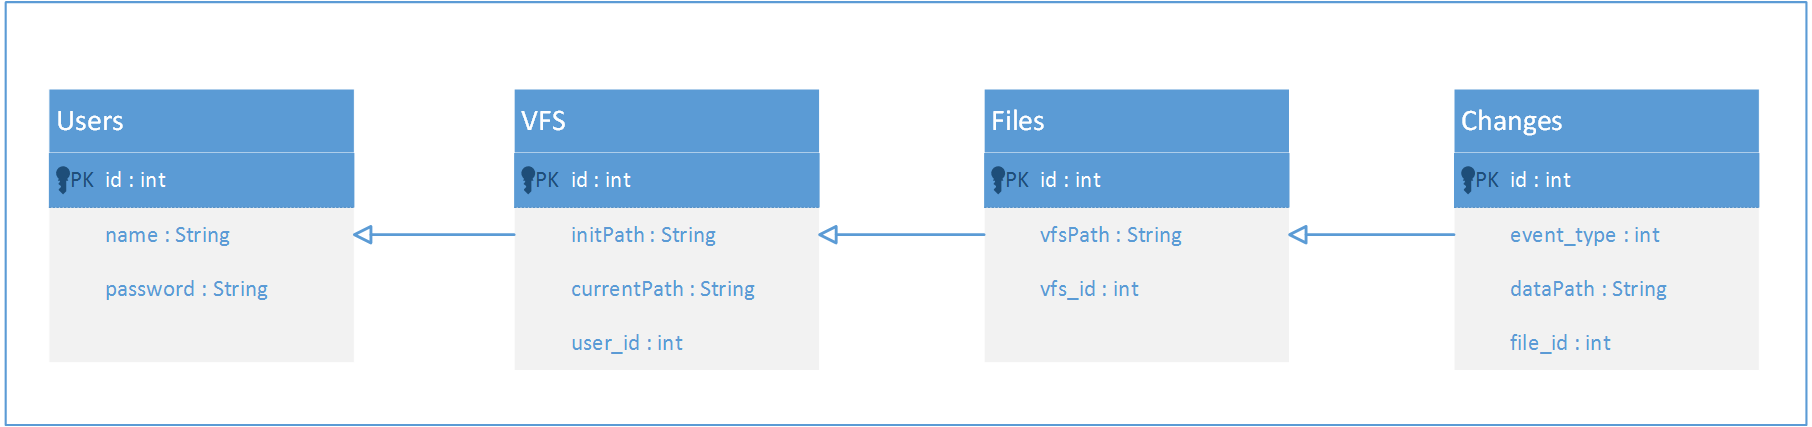
\includegraphics[width=1.00\textwidth]{dbSchema.png}
		\caption{Database Schema}
	\label{fig:dbSchema}
\end{figure}

\noindent One thing to point out is that the server does execute all the changes locally on a current version of the according VFS file. This makes it possible to send the data directly, without having to execute any updates, to a client that would like to retrieve a VFS. 

\subsection{Integration}

\subsubsection{VFS Core}

\subsubsection{Desktop Client}
The obvious thing that had to be changed in the desktop client was the user interface. The controls in the MainForm had to be rearranged a bit since new buttons had to be added and some forms had to be created. The main change in the code basis was to add a layer for the synchronization between the session and the FAT. This means that all method calls from the forms to the session that are going to the FAT object are now going through the synchronizer, which also contains the network connection. 

\subsubsection{Web Client}
Also in the web client new UI elements had to be added, as well as the synchronization layer.



% PART IV: Quick Start Guide
% --------------------------------------

\section{Quick Start Guide}

\subsection{Console Client}
To facilitate debugging we have created a console client. The available commands are described in this section.

\begin{enumerate}
	\item Can be called all the time:
	\begin{itemize}
		\item help: Shows the help text with the available commands.
		\item exit/quit: Exit the client.
	\end{itemize}
	\item Can be called only when NOT mounted:
	\begin{itemize}
		\item create path size: Create a new VFS file at the given path and with the given size.
		\item delete path: Delete the VFS file at the given location.
		\item open path: Open/mount the VFS file at the given location.
	\end{itemize}
	\item Can be called only when a VFS is mounted:
	\begin{itemize}
		\item close: Close the mounted VFS.
		\item ls [path]: List the files/directories in the current or in the given directory.
		\item cd path: Change to the given directory.
		\item rm [-r] path: Remove the given file/directory (recursively with -r).
		\item mk [-p] path size: Make a new file (and parents with -p) of the given size.
		\item mkdir [-p] path: Make a new directory (and parents with -p).
		\item cp source target: Copy the source to the target, both on the VFS.
		\item mv -hv/-vh/-vv source target: Move the source to the target. In the first parameter the first letter indicates the source and the second the target file system.  ‘h’ stands for host and ‘v’ for the virtual. Therefore -hv means import, -vh export and -vv inside the VFS.
		\item rn path newName: Rename the file/directory to the given new name.
		\item size: Show the size of the hole VFS file.
		\item free: Show the free space.
		\item occupied: Show the occupied space.
		\item search [-i] [-a] [-n] filename: Search current directory for the given file (case insensitive with -i, -a search from root, -n non recursive search)
	\end{itemize}
\end{enumerate}


% TODO: Remove this line
%\noindent\textbf{[This part has to be completed by May 13th.]}

% TODO: Remove this text and replace it with actual content
%\emph{Describe how to realize the following use case with your system. Describe the steps involved and how to perform each action (e.g. command line executions and arguments, menu entries, keyboard shortcuts, screenshots). The use case is the following:
%\begin{enumerate}
%\item Start synchronization server on localhost.
%\item Create account on synchronization server.
%\item Create two VFS disks (on the same machine) and link them to the new account.
%\item Import a directory (recursively) from the host file system into Disk 1.
%\item Dispose Disk 1 after the synchronization finished.
%\item Export the directory (recursively) from Disk 2 into the host file system.
%\item Stop synchronization server.
%\end{enumerate}
%}
\subsection{Use Case 1: Import a directory in one and export it in another linked VFS}

\begin{enumerate}
    \item Start vfs.synchronization.server console application without arguments.
    \item Start vfs.clients.desktop GUI application. The app looks like shown in Figure~\ref{fig:basicApp}.
    \item Create a VFS by clicking "Create VFS" in the GUI application.
    \item Open the newly created VFS by clicking "Open VFS" in the GUI application.
    \item Register a new user by clicking "Login", input username and password, and click Register.
    \item You are now logged in.
    \item Click "Synchronize" in order to start synchronizing the VFS with the server.
    \item Find a directory you want to import and drag it on to the GUI application.
    \item Wait for the files to be imported. The app now looks like shown in Figure~\ref{fig:fullApp}.
    \item Click "Close VFS" in order to stop the connection to the server.
    \item Click "Delete VFS" and select the previously created VFS to dispose of it.
    \item Click "Server VFS" and input the previously determined username and password.
    \item Double click the previously synchronized VFS and choose a place to store it.
    \item Click "Open VFS" in order to open the second VFS.
    \item Right click the previously imported folder and click "Export".
		\item The server can now be closed with "exit".
    \item Now choose a place to export the folder to.
    \item Enjoy your exported files!
\end{enumerate}

\subsection{Use Case 2; Automatic FileAdd push}

\begin{enumerate}
    \item Start vfs.synchronization.server console application without arguments.
    \item Start vfs.clients.desktop GUI application.
    \item Create a VFS by clicking "Create VFS" in the GUI application.
    \item Open the newly created VFS by clicking "Open VFS" in the GUI application.
    \item Register a new user by clicking "Login", input username and password, and click Register.
    \item You are now logged in.
    \item Click "Synchronize" in order to start synchronizing the VFS with the server.
    \item Start a second instance of vfs.clients.desktop GUI application.
    \item In the second instance of the GUI application, click "Server VFS" and download the previously synchronized VFS.
    \item In the second instance of the GUI application, click "Open VFS" and open the newly downloaded VFS.
    \item In the second instance of the GUI application, click "Login" and input the chosen username and password.
    \item Create or import a file and/or folder on the first instance of the GUI application.
    \item The files are now pushed to the second GUI application.
		\item The server can now be closed with "exit".
    \item Export the files from the second GUI application.
    \item Enjoy your exported files!
\end{enumerate}

\begin{figure}[H]
	\centering
		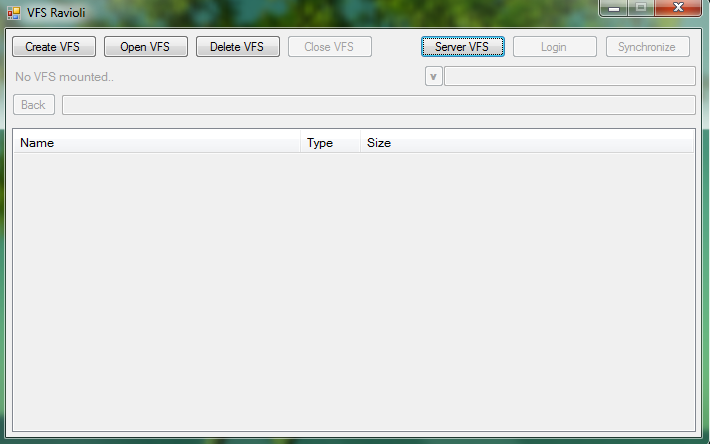
\includegraphics[width=1.00\textwidth]{basicApp.png}
		\caption{Desktop Client after Startup}
	\label{fig:basicApp}
\end{figure}
	
\begin{figure}[H]
	\centering
		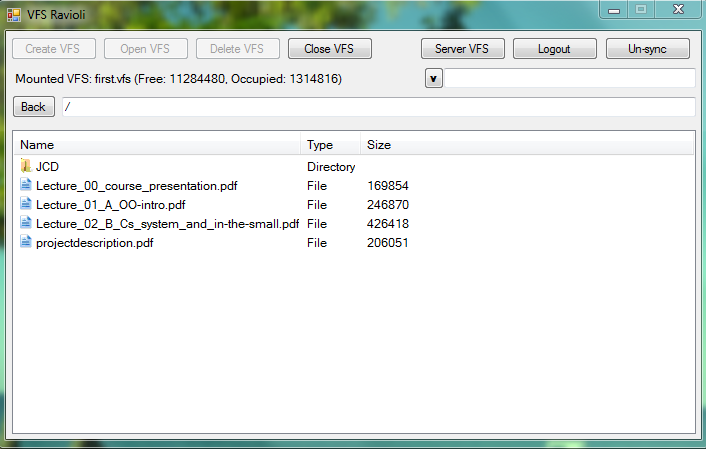
\includegraphics[width=1.00\textwidth]{afterImportApp.png}
		\caption{Desktop Client after Directory Import}
	\label{fig:fullApp}
\end{figure}


\end{document}
